%% ----------------------------------------------------------------
%% Thesis.tex -- MAIN FILE (the one that you compile with LaTeX)
%% ---------------------------------------------------------------- 

% Set up the document
\documentclass[a4paper, 11pt, oneside]{Thesis}  % Use the "Thesis" style, based on the ECS Thesis style by Steve Gunn
\graphicspath{{Figures/}}  % Location of the graphics files (set up for graphics to be in PDF format)

% Include any extra LaTeX packages required
\usepackage[square, numbers, comma, sort&compress]{natbib}  % Use the "Natbib" style for the references in the Bibliography
\usepackage{verbatim}  % Needed for the "comment" environment to make LaTeX comments
\usepackage{vector}  % Allows "\bvec{}" and "\buvec{}" for "blackboard" style bold vectors in maths
\hypersetup{urlcolor=black, colorlinks=true}  % Colours hyperlinks in blue, but this can be distracting if there are many links.
\usepackage{tabularx}
\usepackage{multirow}
\usepackage{wrapfig}
\usepackage{framed}
\usepackage{amssymb}
\usepackage{amsmath}
\usepackage{amsthm}
\usepackage{framed}

%% ----------------------------------------------------------------
\begin{document}
\frontmatter	  % Begin Roman style (i, ii, iii, iv...) page numbering

% Set up the Title Page
\title  {Speculative Loop Parallelization}
\newcommand*{\TITLE}{SPECULATIVE LOOP PARALLELIZATION}
\authors  {\texorpdfstring
            {\href{johannes@jdoerfert.de}{Johannes Doerfert}}
            {Johannes Rudolf Doerfert}
            }
\addresses  {\groupname\\\deptname\\\univname}  % Do not change this here, instead these must be set in the "Thesis.cls" file, please look through it instead
\date       {May 23, 2012}
\subject    {}
\keywords   {}

\maketitle
%% ----------------------------------------------------------------

\setstretch{1.3}  % It is better to have smaller font and larger line spacing than the other way round

% Define the page headers using the FancyHdr package and set up for one-sided printing
\fancyhead{}  % Clears all page headers and footers
\rhead{\thepage}  % Sets the right side header to show the page number
\lhead{}  % Clears the left side page header

\pagestyle{fancy}  % Finally, use the "fancy" page style to implement the FancyHdr headers

%% ----------------------------------------------------------------
% Declaration Page required for the Thesis, your institution may give you a different text to place here
\Declaration{

\addtocontents{toc}{\vspace{1em}}  % Add a gap in the Contents, for aesthetics

\begin{center}
  \bf \large
  Eidesstattliche Erkl\"{a}rung
\end{center}
Ich erkl\"{a}re hiermit an Eides Statt,
dass ich die vorliegende Arbeit selbstst\"{a}ndig verfasst und keine
anderen als die angegebenen Quellen und Hilfsmittel verwendet habe.

\begin{center}
  \bf \large
  Statement in Lieu of an Oath
\end{center}
I hereby confirm that I have written this thesis on my own and 
that I have not used any other media or materials than the ones
referred to in this thesis.

\vfill
\begin{center}
  \bf \large
  Einverst\"{a}ndniserkl\"{a}rung
\end{center}
Ich bin damit einverstanden, dass meine (bestandene) Arbeit in beiden 
Versionen in die Bibliothek der Informatik aufgenommen und damit 
ver\"{o}ffentlicht wird. 

\begin{center}
  \bf \large
  Declaration of Consent
\end{center}
I agree to make both versions of my thesis (with a passing grade) 
accessible to the public by having them added to the library of the
Computer Science Department.

\vfill
\vfill
 
Datum/Date:\\
\rule[1em]{25em}{0.5pt}  % This prints a line to write the date

Unterschrift/Signature:\\
\rule[1em]{25em}{0.5pt}  % This prints a line for the signature
 
}
\clearpage  % Declaration ended, now start a new page

%% ----------------------------------------------------------------
% The "Funny Quote Page"
\pagestyle{empty}  % No headers or footers for the following pages

\null\vfill
% Now comes the "Funny Quote", written in italics
\textit{``Debugging is twice as hard as writing the code in the first place. Therefore, if you write the code as cleverly as possible, you are, by definition, not smart enough to debug it.''}

\begin{flushright}
Brian Kernighan, professor at Princeton University
\end{flushright}

\vfill\vfill\vfill\vfill\vfill\vfill\null
\clearpage  % Funny Quote page ended, start a new page
%% ----------------------------------------------------------------

%\newcommand{\Abstract}{Zusammenfassung}
%% The Abstract Page German
%%\addtotoc{Zusammenfassung}  % Add the "Abstract" page entry to the Contents
%\abstract{
%%\addtocontents{toc}{\vspace{1em}}  % Add a gap in the Contents, for aesthetics

%SPolly, kurz f\"ur spekulatives Polly, ist ein Versuch zwei aktuelle 
%Forschungsprojekte aus dem Bereich des \"Ubersetzerbaus zu kombinieren. 
%Genauer w\"aren das Polly, ein LLVM Projekt um r\"aumliche Datenlokalit\"at und Parallelit\"at
%von regul\"aren Schleifen zu steigern, und Sambamba, welches adaptive Programm\"ubersetzung  erm\"oglicht. Desweiteren geh\"oren Versionsverwaltung, Spekulation
%und Laufzeit Anpassungen zu den Besonderheiten von Sambamba. Als Erweiterung 
%von Polly und mit den M\"oglichkeiten von Sambamba ist SPolly im Stande neuste 
 %Optimierungen und spekulative Parallelisierung auf eine Vielzahl von Schleifen 
 %anzuwenden, sogar bei allgemeinen Anwendungen wie sie zum Beispiel 
 %in der SPEC 2000 Testsammlung zu finden sind. 
 %In solchen Kontexten beinhalten Schleifen
  %nicht (statisch) analysierbare Abh\"angigkeiten und beobachtbare Funktionsaufrufe. 
%Das Potential f\"ur Spekulation h\"angt in solchen F\"allen nicht nur von der 
%Gr\"o\ss{}e der Schleife und der Anzahl der Iterationen ab, sondern auch von der
%Warscheinlichkeit das Abh\"angigkeiten und Funktionsaufrufe auftreten.
%Zusammengefasst findet SPolly vielversprechende Schleifen, parallelisiert diese
%spekulativ und beobachtet das Ergebnis um m\"oglichen Fehlspekulationen entgegenzuwirken.

%Diese Arbeit beschreibt unter welchen Umst\"anden Spekulation m\"oglich ist, 
%wie statische und dynamische Informationen genutzt werden k\"onnen um Fehlspekulationen
%zu vermeiden und wie SPolly sich in die vorhandene Infrastruktur integriert.
%Eine Evaluation mit der SPEC 2000 Testsammlung und verschiedenen
%Versionen des Matrix Multiplikation wird die Ergebnisse und die Vorteile darlegen.

%Diese Arbeit ist in englischer Sprache verfasst.

%}

%\clearpage  % Abstract ended, start a new page

%% ----------------------------------------------------------------
% The Abstract Page
\newcommand{\Abstract}{Abstract}
\addtotoc{Abstract}  % Add the "Abstract" page entry to the Contents
\abstract{
\addtocontents{toc}{\vspace{1em}}  % Add a gap in the Contents, for aesthetics

SPolly, short for speculative Polly, is an attempt to combine two recent research 
projects in the context of compilers. 
There is Polly, an LLVM project to increase data-locality
and parallelism of regular loop nests, and Sambamba, which 
pursues a new, adaptive way of compiling. It offers features like method 
versioning, speculation and runtime adaption. As an extension of the former one
and with the capabilities offered by the latter one,
SPolly can perform state-of-the-art loop optimizations and speculative but sound
loop parallelization on a wide range of loops,
even in general purpose benchmarks as the SPEC 2000 benchmark suite. 
In this context, candidate loops for speculative parallelization may
contain non-computable data dependencies (including possible aliases) 
as well as observable side effects which prohibit  parallelization at first.
The speculative potential of such a candidate loop depends not only on the size and the trip
count, but also on the execution probability of these dependencies and function calls.
Summarized, SPolly detects promising candidate loops, speculatively parallelizes
them and monitors the result to tackle possible misspeculation. 

This thesis will explain under which circumstances speculation is possible,
how static and dynamic information is used to minimize the amount of
misspeculation and how this is integrated into the existing environment of 
Polly and Sambamba. To substantiate the improvements of this work an evaluation on 
SPEC 2000 benchmarks and a case study on different versions of
the matrix multiplication benchmark is presented at the end.

%SPolly, short for speculative Polly, is an attempt to combine two recent research 
%projects in the context of compilers. 
%There is Polly, an LLVM project to increase data-locality
%and parallelism of regular loop nests and Sambamba, which 
%pursues a new, adaptive way of compiling and offers features like method 
%versioning, speculation and runtime adaption. As an extension of the former one
%and with the capabilities offered by the later one,
%SPolly can perform state-of-the-art loop optimizations on a wide range of loops,
%even in general purpose benchmarks as the SPEC 2000 benchmark suite. 
%[CHANGED removed sentence about irreversible function calls an detection of promising loops, added TODO]
%[TODO Should I say something about the ideas for future work ?]
%This thesis will explain under what circumstances speculation is possible,
%how static and dynamic information are used to minimize the amount of
%misspeculation and how this is integrated into the existing environment of 
%Polly and Sambamba. 
%To substantiate the improvements of this work an evaluation on 
%SPEC 2000 benchmarks and a case study on different versions of
%the matrix multiplication benchmark is presented too.


}

\clearpage  % Abstract ended, start a new page
%% ----------------------------------------------------------------

\setstretch{1.3}  % Reset the line-spacing to 1.3 for body text (if it has changed)
\null\vfil
% The Acknowledgements page, for thanking everyone
\acknowledgements{
\addtocontents{toc}{\vspace{1em}}  % Add a gap in the Contents, for aesthetics

  Although I have no ``Loving Wife'' I could thank for keeping the children away,
  there were many friends which helped me to bear the brunt of the work. Especially 
  during the last, indeed frantic days they did their utmost.
  When the only concern is the verging  deadline you may consider yourself lucky
  if you can pass on nearly all other matters. With this in mind it remains to 
  say: Joshua, Ruben and Sarah; Thank you!

  As the daily living is important but not everything when you write your first
  academic contribution, I have to extend special thanks to my advisors. Both of
  them did a heck of a job and endured all my moods and quirks. 
  They were always accessible for questions and helped me in the best possible way 
  during all stages of this work. Furthermore (and in my opinion even more important),
  they encouraged me to structure my work,  something I am admittedly not that good at. 
  From my present view I know it was the best supervision possible.

  Last but not least, I owe special thanks to my supervising professor for the
  liberty he granted me. Even if it took some time to find (or to define) 
  the topic, it was a great experience I would not like to miss. 


}
\clearpage  % End of the Acknowledgements
%% ----------------------------------------------------------------

\pagestyle{fancy}  %The page style headers have been "empty" all this time, now use the "fancy" headers as defined before to bring them back



%% ----------------------------------------------------------------
\lhead{\emph{Contents}}  % Set the left side page header to "Contents"
\dominitoc
\tableofcontents  % Write out the Table of Contents
\clearpage




%% ----------------------------------------------------------------
%\clearpage  % Start a new page
%\lhead{\emph{Physical Constants}}  % Set the left side page header to "Physical Constants"
%\listofconstants{lrcl}  % Include a list of Physical Constants (a four column table)
%{
%% Constant Name & Symbol & = & Constant Value (with units) \\
%Speed of Light & $c$ & $=$ & $2.997\ 924\ 58\times10^{8}\ \mbox{ms}^{-\mbox{s}}$ (exact)\\

%}

%% ----------------------------------------------------------------
%\clearpage  %Start a new page
%\lhead{\emph{Symbols}}  % Set the left side page header to "Symbols"
%\listofnomenclature{lll}  % Include a list of Symbols (a three column table)
%{
%% symbol & name & unit \\
%$a$ & distance & m \\
%$P$ & power & W (Js$^{-1}$) \\
%& & \\ % Gap to separate the Roman symbols from the Greek
%$\omega$ & angular frequency & rads$^{-1}$ \\
%}
%% ----------------------------------------------------------------
% End of the pre-able, contents and lists of things
% Begin the Dedication page

\setstretch{1.3}  % Return the line spacing back to 1.3

\pagestyle{empty}  % Page style needs to be empty for this page
\dedicatory{Dedicated to my father whose never ending patience is priceless.}

\addtocontents{toc}{\vspace{2em}}  % Add a gap in the Contents, for aesthetics


%% ----------------------------------------------------------------
\mainmatter	  % Begin normal, numeric (1,2,3...) page numbering
\pagestyle{fancy}  % Return the page headers back to the "fancy" style

% Include the chapters of the thesis, as separate files
% Just uncomment the lines as you write the chapters
\setcounter{mtc}{4}
% Chapter 1

\chapter{Introduction} % Write in your own chapter title
\label{Chapter1}
\lhead{Chapter 1. \emph{Introduction}} % Write in your own chapter title to set the page header

%\section{Motivation}

Nowadays multiprocessors became ubiquitous even in the area of personal and 
mobile computing; however, automatic parallelization did not. 
Programmers still write sequential code which will be
translated to sequential binaries and executed by a single thread using only
one of many cores. % This kind of execution is still normality. 
Benefits of modern multiprocessors are still unused because neither programmers 
nor compilers may utilize their potential to the full.
Even if legacy applications would be amenable to parallelization, it is unclear 
how to find and exploit theirs potential automatically.  
Apart from the retrieval, parallelism faces the same problems as sequential
code does. Cache invalidation and subsequently cache misses 
caused by poor data-locality is a well known one. 
Heavy research is going on to improve parallelism as well as  data-locality 
but the results may differ.
As there are promising approaches suffering from poor applicability on general 
purpose code, the real problem becomes more and more applying optimizations, not
developing them. 


Techniques using the so called polyhedral model become increasingly popular.
The underlying model is a mathematical description of loop nests with 
their data dependencies. Optimal solutions in terms of e.g., locality or 
parallelism can be derived using this model while it implicitly applies 
traditional optimizations as loop blocking and unrolling. 
Various preliminary results reveal the potential but also the
limits of this technique. Enormous speedups are possible, 
but only for very restricted and therefor few locations.



\section{Related Work}
Research on parallelism and data locality is very popular nowadays, as is the 
polytope model to tackle these problems. With or without speculation, there are
promising attempts all using the polytope model, but the wide range 
impact on general purpose code is still missing.

Tobias Grosser describes in his thesis\cite{grosser:thesis} a speedup of up to
$8$ for the matrix multiplication benchmark, archived by his polyhedral optimizer 
Polly\cite{grosser.11.impact}. He also produced similar results for other
benchmarks of the Polybench\cite{Polybench:Online} benchmark suite. 
Other publications on this 
topic\cite{Bondhugula:2008:PAP:1379022.1375595,BCBPR10,Pradelle:2012:PPB:2086696.2086718} 
show similar results, but they are also limited to the Polybench benchmark suite.
Admittedly, Polybench is well suited for comparative studies, between these 
approaches, but it has less significance for general applicability. 
Baghdadi et. al.\cite{BCBPR10} revealed a huge potential for speculative loop 
optimizations. They state that aggressive loop nest optimizations (including 
parallel execution) are profitable and possible, even though data and flow 
dependencies would statically prevent them. 
Theirs hand made tests also showed 
the impact when different kinds of conflict management are used. 
The results differ from loop to loop as the availability of such conflict 
management systems does. But even if the choice is restricted to one or two, 
their results indicate a general speedup. 




\section{Overview}

SPolly, short for speculative Polly, is an attempt to combine two recent research 
projects in the context of compilers. 
There is Polly, an LLVM project to increase data-locality
and parallelism of regular loop nests and Sambamba, which 
pursues a new, adaptive way of compiling and offers features like method 
versioning, speculation and runtime adaption. As an extension of the former one
and with the capabilities offered by the later one,
SPolly can perform state-of-the-art loop optimizations on a wide range of loops,
even in general purpose benchmarks as the SPEC 2000 benchmark suite. It is also
capable of detection promising loops for parallel execution even if they contain 
irreversibel function calls or non computable dependencies.
This thesis will explain under what circumstances speculation is possible,
how static and dynamic information are used to minimize the amount of
misspeculation and how this is integrated into the existing environment of 
Polly and Sambamba. To substantiate the improvements of this work an evaluation on 
SPEC 2000 benchmarks and a case study on different versions of
the matrix multiplication benchmark is presented at the end.

%The key idea is to enable more loop optimizations by speculation.
%To demarcate this from guessing, profiling is used and combined with 
%static information. The heuristic to choose promising candidates is presented 
%as well as the restrictions  which are weakened or even removed. 


The rest of the thesis will be organised as follows. 
First Chapter \ref{Chapter2} will provide information on the used tools and techniques,
especially Polly and Sambamba. Afterwards the concept as well as the key ideas 
are stated in Chapter \ref{Chapter3}. 
Technical details about SPolly are given in Chapter \ref{Chapter4}, followed by 
an evaluation on the SPEC 2000 and Polybench 3.2 benchmark suites 
(Chapter \ref{Chapter5}). 
While Chapter \ref{Chapter7} concludes the thesis and provides ideas for
future work, a detailed case study on different versions of the matrix 
multiplication example is presented in Chapter \ref{Chapter6}. 

%\vspace*{5mm}
\paragraph*{Note} ~ \\
For simplicity source code is presented in a C like language only.



 % Introduction

% Chapter 2

\chapter{Background} % Write in your own chapter title
\label{Chapter2}
\lhead{Chapter 2. \emph{Background}} % Write in your own chapter title to set the page header

This work takes heavy use of different techniques, theories and tools mostly 
in the context of compiler construction. To simplify the rest of the thesis 
this chapter explains them as far as necessary, thus we may take
them for granted afterwards. As most of the key ideas will suffice, 
some details will be omitted. 
Interested readers have to fall back on the further readings instead. 


\section{LLVM - The Low Level Virtual Machine}
\label{LLVM}
The Low Level Virtual Machine is a compiler infrastructure designed to optimize
during compiletime, linktime and runtime. Originally designed for C and C++, 
many other frontends for a variety of languages exist by now. The source is 
translated into an intermediate representation (LLVM-IR), which is available 
in three different, but equivalent forms. There is the in-memory compiler IR, 
the on-disk bitcode representation and human readable assembly language.
The LLVM-IR is a type-safe, static single assignment based language,
designed for low-level operations. It is capable of 
representing high-level structures in a flexible way.
Due to the fact that LLVM is built in a modular 
way and can be extended easily, most of the state of the art analysis and
optimization techniques are implemented and shipped with LLVM. Plenty of other
extensions, e.g., Polly, can be added by hand. 


\subsection*{Further Reading}

\begin{itemize}
  \item A Compilation Framework for Lifelong Program Analysis \& Transformation
    \cite{LLVM:CGO04}  
  \item \url{http://www.llvm.org} \nocite{LLVM:Online}
\end{itemize}


\clearpage
\section{The Polyhedral Model}
The polyhedral model is a mathematical way to describe the iteration space of 
loop nests, or more likely a very restricted subset of them.
Its became popular as it abstracts from the given source and applies loop
optimizations in a pure mathematical way. Formulating optimization problems 
in terms of linear equations yields an optimal solution with regards to a given
property, e.g., data-locality or parallelism.

%\begin{definition}[Polyhedron] ~\\
  %A polyhedron P in an $n$-dimensional space restricted by $m$ inequalities is defined as:
  %\[ \text{P}:= \{ x \in \mathbb{Z}^n \, |\, Ax\leq b \text{ where $A\in\mathbb{Z}^{m*n} $ and $ b\in\mathbb{Z}^{m}$ are constant } \} \]
  %\label{def:polyhedron}
%\end{definition}



%\lstset{frame=none}
%\begin{wrapfigure}[]{l}{0.4\textwidth}
  %\vspace*{-5mm}
  %\subfloat[Example loop nest]{%
    %\begin{minipage}[c][0.6\width]{%
           %0.35\textwidth}
           %\centering%
      %\lstinputlisting{Primitives/Code/Polytope2d.c}
      %\label{lst:Polytope2dC}
    %\end{minipage}
  %} 
  
  %\subfloat[Iteration space for listing \ref{lst:Polytope2dC}]{%
    %\begin{minipage}[c][1.2\width]{%
           %0.35\textwidth}
           %\centering%
      %\includegraphics[width=0.9\textwidth]{Figures/Polytope2d.eps}
      %\label{lst:Polytope2dPolyhedral}
    %\end{minipage}
  %}


  %\caption{The polytope model in action }
  %\label{fig:Polyhedron2d}
%\end{wrapfigure}
%\resetlst
Within the polyhedral model the iteration space is represented as a $\mathbb{Z}$-polyhedron,
simply spoken a geometric object with flat surfaces existing in a space of 
any general dimension. To do so, it is necessary that the iteration space 
can be described as solution set of affine inequalities
(equation \ref{eq:IterationSpace}), where the loop bounds are encoded in a translation
($b$) and the steppings in a matrix ($A$). 
\begin{equation}
  \text{Iteration Space IS } := \{ x \in \mathbb{Z}^n \, |\, Ax\leq b \text{ with $A\in\mathbb{Z}^{m*n} $, $ b\in\mathbb{Z}^{m}$  } \} \label{eq:IterationSpace}
\end{equation}
%Definition \ref{def:polyhedron} restrict all (integer) points within the polyhedron
%to be solutions of an affine system of inequalities which can be derived from
%the source code. The example in figure \ref{fig:Polytope2d} shows how these 
%inequalities (figure \ref{lst:Polytope2dInequalities}) 
%are derived from the source presented in listing \ref{lst:Polytope2dC} and how 
%the resulting polyhedral (figure \ref{lst:Polytope2dPolyhedral}) looks like.
%[TODO unify the two examples]

%For clarification it is worth to say
%that some authors e.g., Benabderrahmane et al. \cite{BPCB10} use the term 
%polyhedron instead of polytope. 
%As each loop corresponds to a dimension of the vector space the
%dimension of the polyhedron is determined by the depth of the loop nest. 
In addition to the points of the iteration space, the polyhedral model is also
capable of representing loop carried dependencies between two iterations. 
Figure \ref{fig:ExampleLoopNest} illustrates this by relating a simple loop 
nest({\footnotesize A}) to its representation within the polyhedral 
model({\footnotesize B}). 
%The main benefit of 
%this representation is that transformations can be done in an optimal manner
%using an integer linear programming solver which maximizes the loop nest for 
%e.g., parallelism.
An optmization within the model (which is in fact a composed
affine transformation) could yield 
%with the additional advantage that they implicitly apply 
%traditional loop optimizations including tiling, skewing, loop interchange and
%unrolling. 
%Using the example in listing \ref{lst:ExampleLoopNest} again we may end up with
a loop nest as presented in listing \ref{lst:ExampleLoopNestTransformed}. 

Data-locality has been increased by introducing the two inner most loops which
also remove the data dependency from the outer most one, 
thus the whole loope nest may be executed in parallel now.

\lstset{frame=none}
\begin{figure}[htbp]
  \centering
  \subfloat[Simple loop nest]{%
    \begin{minipage}[c][0.6\width]{%
           0.45\textwidth}
           \centering%
    \lstinputlisting{Primitives/Code/ExampleLoopNest.c}
    \label{lst:ExampleLoopNest}
    \end{minipage}
  } 
  \subfloat[Polyhedral representation for listing \ref{lst:ExampleLoopNest}]{%
    \begin{minipage}[c][0.6\width]{%
           0.45\textwidth}
           \centering%
    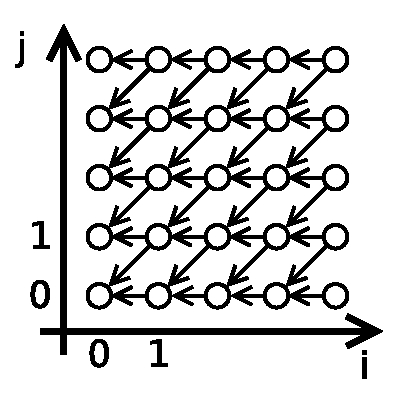
\includegraphics[width=0.55\textwidth]{Figures/ExampleLoopNestPolytope2.eps}
    \label{fig:ExampleLoopNestPolytope}
    \end{minipage}
  }
  
  \subfloat[Optimized version of listing \ref{lst:ExampleLoopNest}]{%
    \lstinputlisting{Primitives/Code/ExampleLoopNestTransformed.c}
    \label{lst:ExampleLoopNestTransformed} 
  }
  \caption{An example loop nest with its polyhedral representation}
  \label{fig:ExampleLoopNest}
\end{figure}
\resetlst



\lstset{frame=none}
\begin{figure}[htbp]
  \centering
\end{figure}
\resetlst

\subsection*{Further Reading}
\begin{itemize}
  \item The Polyhedral Model is More Widely Applicable Than Yoy Think \cite{BPCB10}
  \item Loop Parallelization in the Polytope Model \cite{Lengauer93loopparallelization}  
  \item A practical automatic polyhedral parallelizer and locality optimizer \cite{Bondhugula:2008:PAP:1379022.1375595}
  \item PoCC - The Polyhedral Compiler Collection \cite{PoCC:Online}
  \item Polyhedral parallelization of binary code \cite{Pradelle:2012:PPB:2086696.2086718}
  \item Putting Polyhedral Loop Transformations to Work \cite{BCGST03} 
\end{itemize}

\clearpage

\section{Polly - A Polyhedral Optimizer For LLVM}
\label{Polly}
Exploiting parallelism and data-locality in order to balance the work load
and to improve cache utilization are the main goals of the Polly research project.
The polyhedral model is used as abstract mathematical representation to get optimal
results for a particular objective. The three-step approach of Polly first detects
maximal loop nests suitable for polyhedral representation. These representations
are analyzed and transformed before they are converted to code (here LLVM-IR)
again. In the case of Polly the code generation is capable of generating thread 
level parallelism and vector instructions. The code regions Polly is interested 
in, are called static control parts, or short SCoPs. Such a SCoP is 
the most central entity within Polly and crucial for any kind of argumentation.
%Apart from the
%following descriptions figure \ref{fig:PollyArchitecture} provides an overview
%of the architecture of Polly.

\begin{definition}[Affine Transformation] ~\\
  Affine transformations are linear transformations followed by a translations,
  thus they can be written as:
  \[ f(x_1,\dots,x_n) := A_1\, x_1 + \dots + A_n\, x_n + b\]

  \label{def:AffineTransformation}
\end{definition}

\begin{definition}[Canonical Induction Variable] ~\\
  An induction variable is canonical if it start at zero and steps by one.
  \label{def:CanonicalInductionVariable}
\end{definition}

\subsection{Static Control Parts}
%\begin{wrapfigure}[]{r}{0.15\textwidth}
  %\centering
  %%\vspace*{-5mm}
  %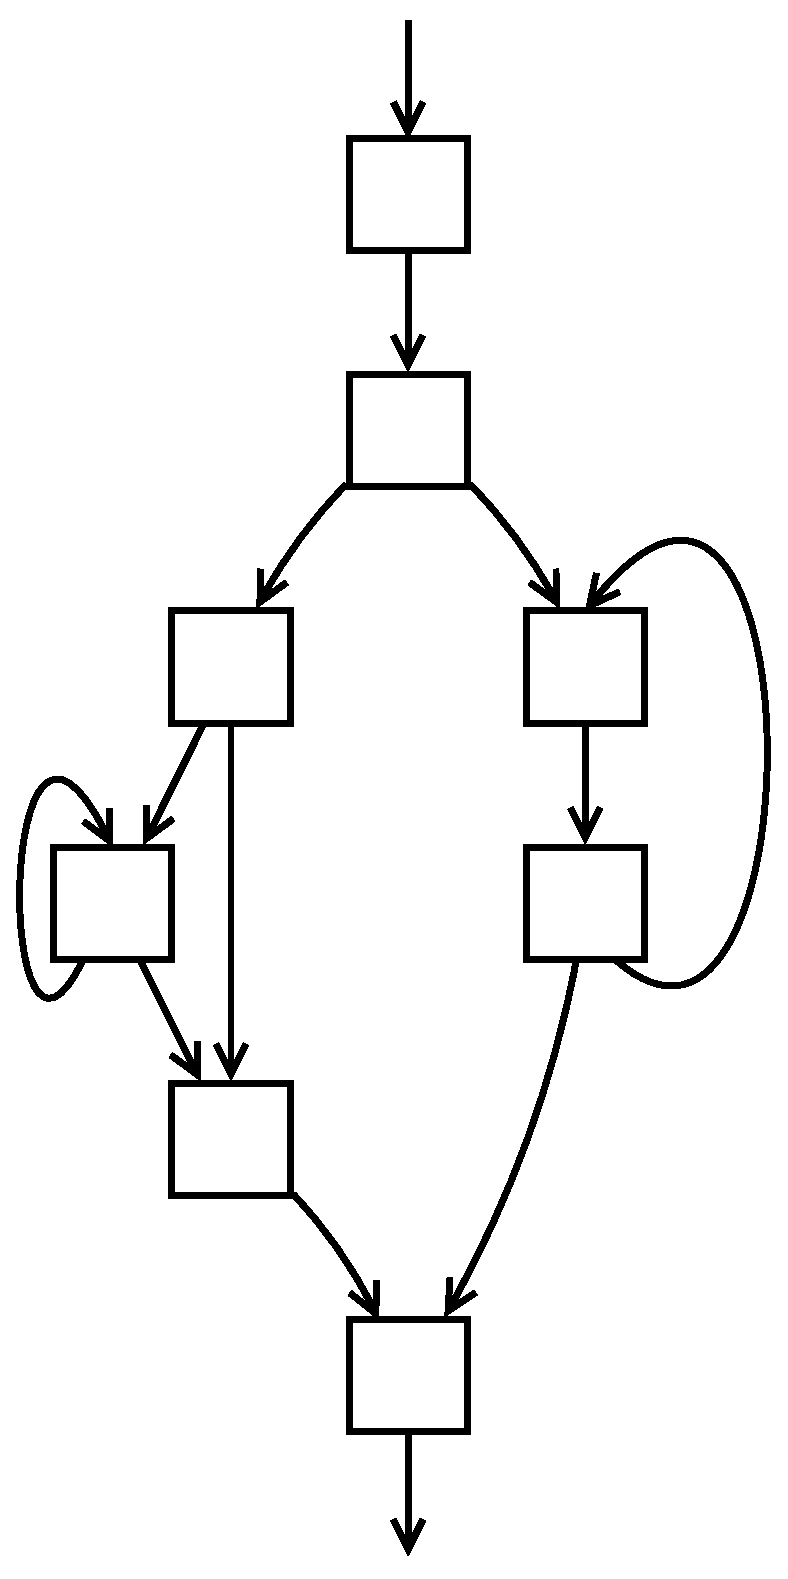
\includegraphics[width=0.15\textwidth]{SimpleRegionCFG.eps}
  %\caption{SCoP CFG}
  %\label{fig:PossibleSCoPCFG}  
%\end{wrapfigure}
A static control part is a region with statically known control flow and memory
accesses. As part of the control flow graph it is restricted to have one entry
edge and one exit edge while within loops and conditionals are allowed inside.
To predict all accesses, it is necessary to restrict loop bounds and branch 
conditions to be affine with respect to invariant parameters 
and surrounding iteration variables, but only if they are canonical. 
Because memory accesses are a crucial for data flow information,
SCoPs are not allowed to contain aliasing instructions at all. 
Furthermore only affine access functions will yield an precise result as 
non affine ones are overestimated (but not forbidden per se).
The last point concerns called function as only pure functional ones are allowed
here.
%Figure \ref{fig:PossibleSCoPCFG} shows the CFG of SCoP 

While some of these conditions (e.g., the canonical induction variables) 
can be achieved through preprocessing, the remaining ones are still 
quite restrictive. The desired result, namely the SCoPs, are valuable because
they can be represented within the polyhedral model, thus further analyses and
transformations are not restricted to the particular source code anymore.

Although all regions fulfilling these requirements are
technically SCoPs, we will restrict ourself to those containing at least one loop.

%\begin{table}[htbp] 
  %\centering
  %\caption{Restrictions on SCoPs}
    %\begin{itemize}
      %\item Only nested loops and conditionals
      %\item Only branches with affine conditions
      %\item Only affine accesses based on a constant pointer
      %\item No unsigned iteration variables \footnote{}
      %\item No aliasing instructions
      %\item Only canonical PHI nodes and induction variables
      %\item Instructions may not be used in PHI nodes outside the region\footnotemark[1]
      %\item Only ``readnone'' function calls
      %\item No alloca or cast instructions within the region
      %\item Only affine trip counts for loops
      %\item No PHI nodes in the region exit block
      %\item Only simple regions not containing the entry block of the function
      %%\item \textit{A SCoP should contain at least one loop}
    %\end{itemize}
    %\flushleft{\footnotemark[1] open for further work }
  %\label{tab:SCoPConstraints}
%\end{table}



\subsection{SCoP Detection}
Pollys SCoP detection is the gateway to all further analyzses and 
transformations. All regions fulfilling the properties described in the 
last section, or in short, all (valid) SCoPs are detected here. 
The special interest of this part arises from the fact that all 
regions declared as valid SCoPs will be considered for pollyhedral 
optimizations. Almost regardless of theirs content, any region could be given to
Polly if the SCoP detection is properly instrumented. Two important consequences
can be derived and summarized as:
Utilizing the strength of Polly is possible in much more situations as 
intentionally implemented but coupled with responsibility of the outcome.

\subsection{Loop Optimizations}
Polly uses the integer set library (isl) to compute the scheduling and
tiling for a SCoP. Once the polyhedral representation is computed,
an optimized version of the  algorithm proposed by Bondhugula et 
al.\cite{Bondhugula:2008:PAP:1379022.1375595}
will compute a new scheduling and tiling scheme. 
Traditional loop optimizations such as blocking, interchange, splitting,
unrolling or unswitching are implicitly applied during this step. 
%Not only the new scheduling but also the new data dependencies are computed, 
%crucial to exploit parallelism.
%Based on these dependencies parallelism is exploited as explained in the next section. 

%\textit{The loop optimizations offers many possibilities in the context 
%of Sambamba (see \ref{FurtherWorkISL}).}


\subsubsection{Parallel Code Generation}
While cache locality is implicitly improved by rescheduling and tiling 
of the loop nest,  parallel code needs to be generated explicitly afterwards.
Polly is capable of generating
thread level parallelism using OpenMP annotations and data level parallelism 
using SIMD instructions. 
%The former one depends on the OpenMP shared library 
%being present while the later one uses the LLVM built-in vector instruction.
If the former one is desired, the first loop without any loop carried 
dependencies will be rewritten as if there were OpenMP annotations in the first
place. Enabling the later one, namely vector code generation 
will not only try to vectorize the innermost loop but also the 
scheduling is changed to allow this more often.

%\begin{figure}[htbp]
  %\centering
  %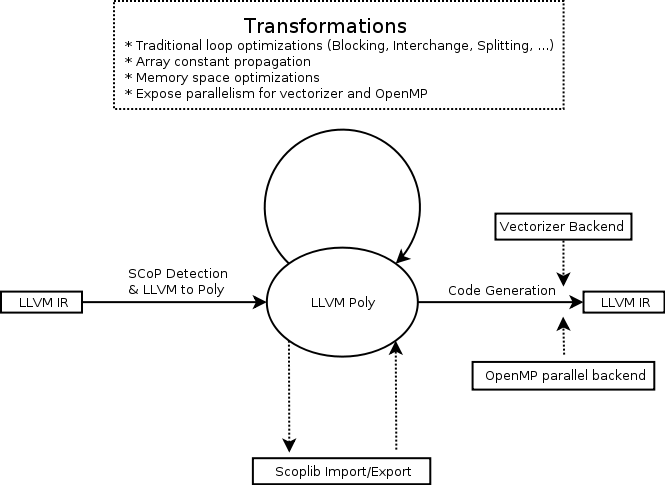
\includegraphics[width=0.9\textwidth]{architecture.png}
  %\caption{Pollys architecture \cite{Polly:Online}}
  %\label{fig:PollyArchitecture}  
%\end{figure}


\subsection*{Further Reading}

\begin{itemize}
  \item Polly - Polyhedral optimization in LLVM \cite{grosser.11.impact}  
  \item Enabling Polyhedral Optimizations in LLVM \cite{grosser:thesis}
  %\item A Framework for Automatic OpenMP Code Generation \cite{raghesh2011framework}
  \item Base algorithm of isl \cite{Bondhugula:2008:PAP:1379022.1375595}
  \item \url{http://polly.llvm.org} \nocite{Polly:Online}
  \item \url{http://www.kotnet.org/~skimo/isl/} \nocite{ISL:Online}
\end{itemize}





\clearpage
\phantomsection
\section*{2.4 ~ Sambamba \\ A Framework For Adaptive Program Optimization}
\addcontentsline{toc}{section}{2.4 ~ Sambamba - A Framework For Adaptive Program Optimization} 
The Sambamba project is build on top of the LLVM compiler infrastructure and 
aims at adaptive and speculative runtime optimizations.
Dynamic information about arguments or the global state may allow optimization
which could not be applied at compile 
\begin{wrapfigure}[]{r}{0.3\textwidth}
  \centering
  %\vspace*{-5mm}
  \includegraphics[width=0.3\textwidth]{SambambaConcept.eps}
  \caption{Sambamba in a nutshell}
  \label{fig:SambambaConcept}  
\end{wrapfigure}
time or did not seem interesting back then. It is easily extendible with 
compile time and a runtime parts. While each one is conceptually 
independent, the compile time parts may store information which can be accessed
at runtime to reduce the overhead, even if expensive analysis results are needed. 
Another fundamental pillar of the framework is the multi versioning system which
allows for different, specialized function versions.
[TODO FILL THIS PAGE ]
%[TODO should VMAD be mentioned here]
%A similar approach has
%been published by Jimborean et al.\cite{JIMBOREAN-2012-664345}, in fact th
%In both cases a dispatcher is used to choose one of the available 
%implementations each time the function is called. 
%In this manner exclusive optimizations can be applied on the same function and
%according to the input a version can be dispatched. Runtime profiling also 
%reveals opportunities to speculatively transform the program and obtain more
%specialized versions. A main difference between Sambamba and the work of 
%Jimborean is probably how these function versions are constructed. Sambamba does
%not rely on source code annotations but allows all modules to find and extract
%the versions fully automatic. 
A high level view on the Sambama concept is given
by figure \ref{fig:SambambaConcept} before some of the  built-in utilities 
and modules, used during this work, are explained. 


\clearpage
\subsection{Sambambas Parallelizer}
\begin{wrapfigure}[]{l}{0.40\textwidth}
  \centering
  %\vspace*{-10mm}
  \includegraphics[width=0.38\textwidth]{TransactionQueue.eps}
  \caption{Symboliced transaction queue with 3 worker threads}
  \label{fig:TransactionQueue}  
\end{wrapfigure}
The Sambamba parallelizer will become the main interface for any kind of 
parallelization in the framework. At the moment it is in need of parallel control
flow graphs to explicitly state section which should be executed in parallel, but
in the future more automatic loop parallelization will be implemented too. 
The runtime part of the parallelizer instantiates its own worker threads so there
is no need for external libraries (as OpenMP) in order to execute tasks in parallel. \\


\subsection{Parallel Control Flow Graphs}
\begin{wrapfigure}[]{r}{0.35\textwidth}
  \centering
  \vspace*{-5mm}
  \begin{minipage}[c][0.37\width]{\textwidth}
  \includegraphics[width=0.33\textwidth]{ParallelSectionEx.eps}
  \end{minipage}
  \caption{A parallel section with 3 transactions}
  \label{fig:ParallelSectionEx}  
\end{wrapfigure}
A parallel control flow graph (ParCFG) is a data structure used by the
parallelizer to express parallel sections within an ordinary CFG. 
Each parallel sections consist of an entry block called \texttt{piStart} and
an exit block called \texttt{piEnd}. The \texttt{piStart} is terminated by a 
symbolic switch statement which may have an arbitrary number of predecessors. 
Every predecessor denotes a, so called, transaction which ends in the 
\texttt{piEnd} block after some arbitrary computation. 
Once parallelized each transaction may be executed.
Figure \ref{fig:ParallelSectionEx} shows such a parallel section with 3 
transactions. 


\subsection*{Further Reading}
\begin{itemize}
  \item Sambamba: A Runtime System for Online Adaptive Parallelization \cite{DBLP:conf/cc/StreitHZH12}  
  \item \url{http://www.sambamba.org} \nocite{StreitHZH12:Online}
\end{itemize}



 % Background Theory 

% Chapter 3

\chapter{Concept} % Write in your own chapter title
\label{Chapter3}
\lhead{Chapter 3. \emph{Concept}} % Write in your own chapter title to set the page header

From a high point of view, this work tries to weaken the harsh requirements on 
SCoPs in order to make Pollys loop analyses and optimizations applicable on a 
wider range of programs. We expect benefit not only from the polyhedral 
optimizations, but also through speculative parallelization. The polyhedral 
analyses are used twice since they reveal loop nests which may be optimized as 
well as speculatively parallelizeable loops. 
Apart from the implementation work, which will be described in the 
next chapter, immense effort has been made on the concepts and key ideas behind.
We believe that these ideas and the knowledge gained during the work is very 
valuable not only for future work on SPolly or one of its bases but also for
other approaches facing similar situations.
%On the way to a working version 
%many pitfalls have been encountered that should be avoided in the future, 
%perhaps with similar approaches we worked out. 


\section{SPolly In A Nutshell}
%SPolly, as presented here, is composed of a compile time and a runtime part. 
%Their respective tasks are related but not the same. During both steps the, so
%called, region speculation is used to interact with Polly. 
%It is also the 
%part of SPolly which is not integrated  into the Sambamba framework. As some
%of the functionalities do not rely on speculation, it is possible to integrate
%them into the main application of Polly anytime soon. 

%\paragraph{Compile Time }~\\
\begin{wrapfigure}[]{r}{0.5\textwidth}
  \centering
  \includegraphics[width=0.5\textwidth]{Figures/draftPaperCT.eps}
  \caption{Draft paper: \\SPolly at compile time}
  \vspace*{-5mm}
  \label{fig:draftPaperCT}  
\end{wrapfigure}
During \textbf{compile time} the main goal of SPolly is to simplify the runtime part, thus
to reduce runtime overhead through preprocessing and even static method versioning.
First  the SCoP detection tries to find valid regions within the given LLVM-IR, 
but instead of rejecting a region once a restriction is violated, 
the region speculation is asked how to proceed. Restrictions we want to speculate
on are gathered by the region speculation, but ignored by the SCoP detection.
This proceeding allows to find all violations with a region and to treat valid and
speculatively valid ones nearly the same. After all  
speculative valid SCoPs (or short sSCoPs) are encountered the Sambamba compile 
time part takes action. It separates the sSCoPs as some of them do not really 
need speculation at all. Those sSCoPs are optimized and exchanged, 
while the others are currently only extracted. This means they are replaced by
calls to functions only containing the speculative valid region. 
%(see \ref{RegionExtraction}).
At the moment, no pre computation takes place and the onliest violations 
not dependent on speculation are special kinds of aliasing instructions, 
namely those which can be ruled out by tests in beforehand. 
%Further details on
%the ratings are given in section \ref{RegionScores} while 
%section \ref{SpeculationFreesSCoPs} coveres the case of speculation free sSCoPs.

%\paragraph{Runtime }~\\
\begin{wrapfigure}[]{l}{0.5\textwidth}
  \centering
  \includegraphics[width=0.5\textwidth]{Figures/draftPaperRT.eps}
  \caption{Draft paper: \\ SPolly at runtime}
  \vspace*{-5mm}
  \label{fig:draftPaperCT}  
\end{wrapfigure}
The \textbf{runtime} part of SPolly first retrieves the extracted sSCoPs and 
precomputed versions from the data store. If not already done during  compile
time, profiling versions will be created now. It would be possible to restrict
this to the best rated sSCoPs only, but as the creation is very cheap and the execution 
overhead for most of them non-existent it is feasible to do so for rather bad
ranked sSCoPs as well. Those profiling versions will now collect information
not only about the time consumption of the sSCoP, but also about loop bounds,
branch probabilities and the results of introduced checks. Except of the time
consumption these values will affect the rating of the sSCoP which again is used
to identify promising sSCoPs. The next section
will explain this rating and the effects of profiling in more detail, while
section \ref{IntroducedTests} covers the test creation and theirs use. 
As explained above, the combined static and dynamic information determine which region
is promising, thus which region will be speculatively optimized and in the end
executed in parallel. Because the impact on the performance might be worse than
expected, maybe even worse than in the beginning, the runtime part will
continually monitor all exchanged functions and intervene if necessary. As the
method versioning of Sambamba is not fully evolved, SPolly will not try to create
different optimized versions based on different parameters even if this would be
already possible. 


\section{Region Scores}
\label{RegionScores}
\lstset{frame=none}
\begin{figure}[h]
  %{r}{0.4\textwidth}
  \centering
  \subfloat[Complete static sSCoP]{
    \begin{minipage}[c][3cm]{0.45\textwidth}
      \lstinputlisting{Primitives/Code/sSCoPstatic.c}
      \label{lst:sSCoPstatic}  
    \end{minipage}
  }
  \subfloat[sSCoP with variable loop bounds and a function call]{
    \begin{minipage}[c][3cm]{0.45\textwidth}
      \lstinputlisting{Primitives/Code/sSCoPbounds.c}
      \label{lst:sSCoPcall}  
    \end{minipage}
  }

  \subfloat[Branch within a sSCoP]{
    \begin{minipage}[c][3cm]{0.45\textwidth}
      \lstinputlisting{Primitives/Code/sSCoPbranch.c}
      \label{lst:sSCoPbranch}  
    \end{minipage}
  }
  \subfloat[irreversible call within a sSCoP]{
    \begin{minipage}[c][3cm]{0.45\textwidth}
      \lstinputlisting{Primitives/Code/sSCoPprintf.c}
      \label{lst:sSCoPprintf}  
    \end{minipage}
  }
  \caption{example sSCoPs}
  \label{fig:ScoredSCoPs}
\end{figure}
\resetlst

Region scores are used as a heuristic to decide whether or not a sSCoP is worth
to speculate on, thus for which regions profiling and optimized versions should
be created and as a result executed.
As the former ones may change the score again it is reasonable to create 
optimized versions only if the profiling results suggest to do so. 
It is obvious that we want to consider only loops and loop nests of a certain size,
thus profiling the trip count may have a enormous impact on the actual region score.
Additionally we are interested in execution paths within a sSCoP in order to predict how often
e.g., irreversible instructions, may be executed. While such instructions, like
calls of \texttt{printf}, may cause STM rollbacks during the parallel executions, 
branch probabilities may also have a huge impact on the actual sSCoP size and
only rarely occurring dependencies. 
To clarify the idea,  the regions scores for the listings \ref{lst:sSCoPstatic}
to \ref{lst:sSCoPprintf} as well as some other listings contained in this 
thesis is listed in table \ref{tab:Scores}. For a detailed explanation on the 
implementation and meaning see the corresponding section in the next chapter. 

\begin{table}[htbp]
  \centering
  \caption{Scores for the sSCoPs presented in various listings}
  \begin{tabular}{ c l}
    listing & score \\
    \hline
    \ref{lst:ExampleLoopNest} & $ 408 $ \\
    \ref{lst:sSCoPstatic} & $ 576 $ \\
    %\hfill \text{  (if \texttt{A,B} and \texttt{C} may alias)} $ \\
    \ref{lst:sSCoPbranch} & $63 * (11 + ((7 * \text{@if.then\_ex\_prob}) / 100) + ((5 * \text{@if.else\_ex\_prob}) / 100)) $ \\
    \ref{lst:sSCoPcall} & $((0 \text{ smax \%N}) / 16) * (7 + (10 * ((0 \text{ smax \%M}) / 16)))$ \\ 
    \ref{lst:sSCoPprintf} & $((0\text{ smax }\%\text{N}) / 16) * (6 + (-1000 * \text{@if.then\_ex\_prob} / 100)$ \\
    \ref{lst:AliastestAccessesSrc} & $  (7 + ((8 + (8 * (\%\text{N} / 16))) * (\%\text{N} / 16))) * ((0\text{ smax \%N}) / 16) $ \\

   \end{tabular}
  \label{tab:Scores}
\end{table}



\section{Method Versioning}
Even if method versioning in Sambamba is not fully implement yet, SPolly is 
already capable of generating a profiling and an optimized version. Both just 
transform the sSCoP, thus only the loop or loop nest has to be cloned and stored.
Further work on SPolly will include the creation of more different optimized 
versions as there are plenty of optional parameters which could be adjusted as 
needed. The impact of tiling size, loop fusion and the amount of actual introduced
tests for the optimized version may have significant impact, but in the short time
of this work it was not feasible to investigate them fully.


\section{Introduced Tests}
\label{IntroducedTests}
The mentioned tests are one attempt to keep down the rate of misspeculations. 
First of all they are used to refine region scores in the context of profiling 
but they can be of great use in optimized versions too. At the moment SPolly is
capable of creating two different kind of checks, which may partially rule out
SCoP violations completely. If so we may call the tests complete and we apply 
them on the optimized version with no need of speculate at all. As such cases can 
improve the applicability of Polly even without an STM, they could find their 
way into the main branch one day. At this point we take advantage of Pollys
default behaviour which is to copy the optimized SCoP as an alternative to the
original one. Figure \ref{fig:PollySCoPCFG} shows the CFG after Polly optimized
a given SCoP. The dotted edge is not taken since the guard of the conditional is
constant true, but in the SPolly version it is replaced by the actual test result 
(see figure \ref{SPollySCoPCFG}).

\begin{figure}[htbp]
  \centering
  \subfloat[CFG after optimization with Polly]{
    \begin{minipage}[c][1\width]{0.5\textwidth}
    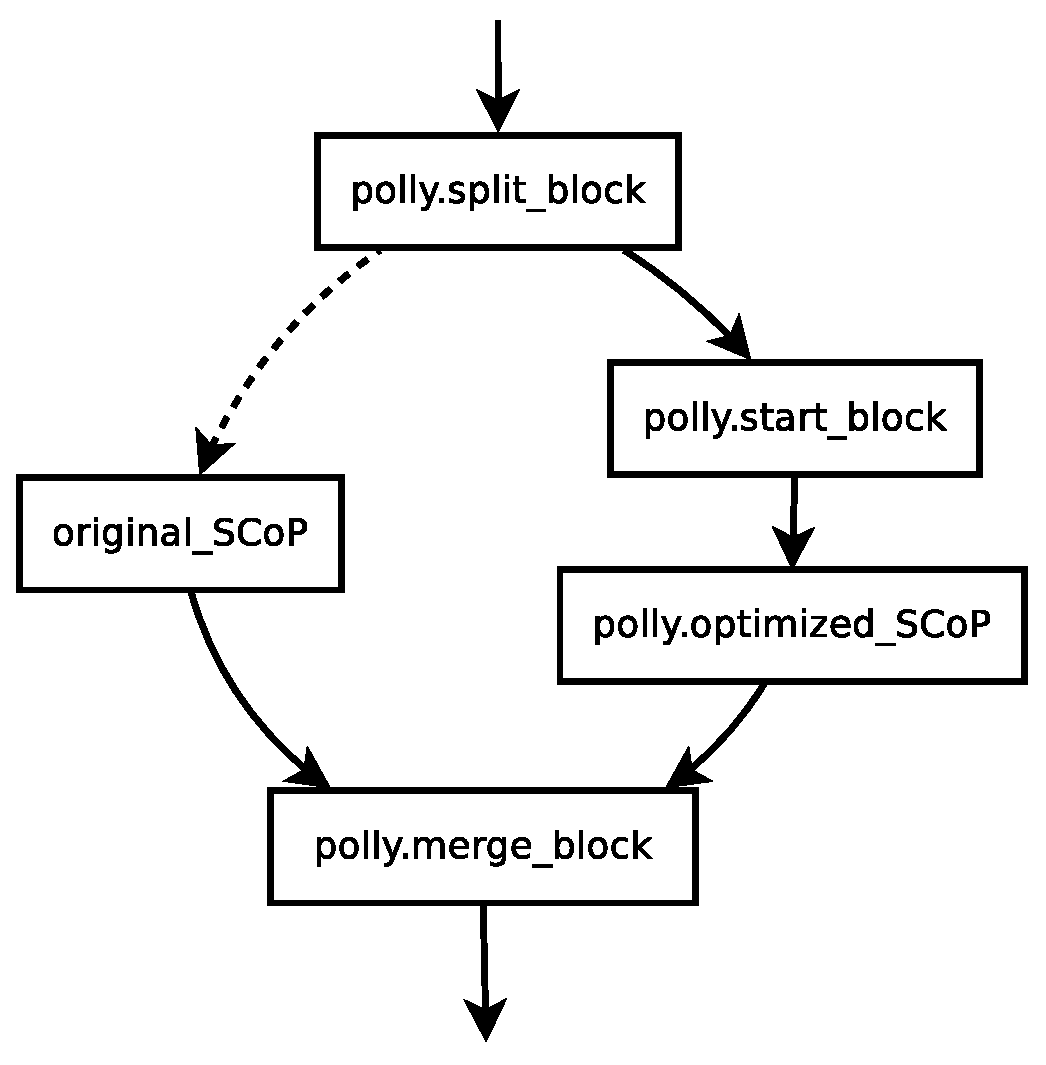
\includegraphics[width=0.9\textwidth]{Figures/PollySCoPCFG.eps}
    \label{fig:PollySCoPCFG}
    \end{minipage}
  }
  \subfloat[CFG after optimization with SPolly]{
    \begin{minipage}[c][1\width]{0.5\textwidth}
    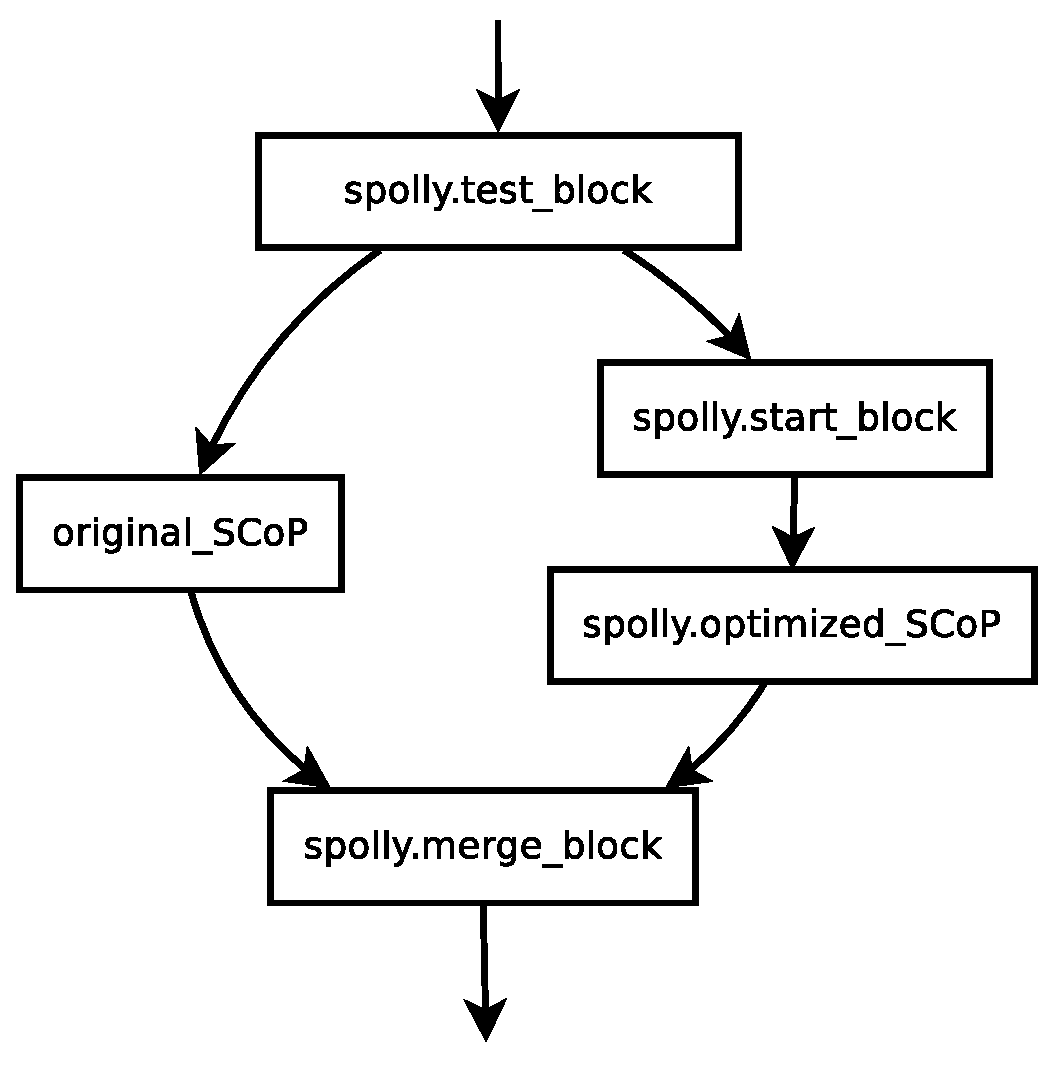
\includegraphics[width=0.9\textwidth]{Figures/SPollySCoPCFG.eps}
    \label{fig:SPollySCoPCFG}
    \end{minipage}
  }
  \caption{CFG produced by Polly and SPolly, respectively}
  \label{fig:SCoPCFG}  
\end{figure}

\subsection{Alias Tests}
Testing for aliasing pointers in general would not be feasible so another way 
was chosen. Only sSCoP invariant pointers are tested once before the sSCoP is
entered. If the test succeeds, thus no aliases are found, the optimized version
is executed. At compile time the accesses for each base pointer are collected and
marked either as possible minimal, possible maximal or not interesting access. At 
runtime all possible minimal and maximal accesses are respectively compared until,
in the end, the minimal and the maximal access for each base pointer is computed.
The alias test as such compares again the minimal access for a base pointer with the maximal 
accesses for each other base pointer and vice versa. After this comparison chain the 
result may indicate or rule out aliasing between them. As Polly introduces two 
versions of a SCoP by default, we may just replaces the constant guard in the
split block in order to choose the executed version based on the test result.
If all base pointers are invariant in the SCoP the test is complete,
thus aliasing can be ruled out for the sSCoP at runtime.
However, non invariant pointers are not tested at all, as it would 
imply to perform all computation and testing within the loop. 
Figure \ref{fig:AliastestConcept} illustrates the concept of the alias
tests while listing \ref{lst:AliastestAccessesSrc} and figure
\ref{fig:AliastestAccesses} provide an example loop nest and the corresponding 
minimal and maximal memory accesses. 
The alias test for this example would look like listing
\ref{lst:AliastestAccessesOut}.

\lstset{frame=none}
\begin{figure}[htbp]
  \centering
  \subfloat[Alias test from a birds eye view]{
  \begin{minipage}[c][4cm]{\textwidth}
    \includegraphics[width=0.9\textwidth]{Primitives/aliastest.eps}
  \end{minipage}
  \label{fig:AliastestConcept}  
  }

  \vspace*{5mm}
  \subfloat[Aliasing accesses]{
    \begin{minipage}[c][4cm]{0.5\textwidth}
    \lstinputlisting{Primitives/Code/aliastestbsp.c}
    \end{minipage}
    \label{lst:AliastestAccessesSrc}  
  }
  \subfloat[Statically derived min/maximal accesses]{
    \begin{minipage}[c][4cm]{0.4\textwidth}
    \vspace*{-2mm}
    \centering
    \begin{tabular}{ c c c c }
      Acc & bp & ma & Ma \\
      \hline
      I1 & C & 0 & N$ * $N$ - 1$ \\ 
      I2 & C & 0 & N$ * $N$ - 1$\\ 
      I3 & A & 0 & N$ * $N$ - 1$\\ 
      I4 & B & 0 & N$ * $N$ - 1$\\ 
    \end{tabular}
    \end{minipage}
    \label{fig:AliastestAccesses}  
  }
  
  \subfloat[Introduced compare chain]{
      \lstinputlisting{Primitives/Code/aliastestout.c}
    \label{lst:AliastestAccessesOut}  
  }
  \caption{Alias tests concept and example}
  \label{fig:Aliastest}  
\end{figure}
\resetlst




\subsection{Invariant Tests}
Apart from alias tests, SPolly may introduce invariants tests if there are
possibly invariant variables and a function call within a sSCoP. The key idea
is to monitor possible changes in such variables during the execution of the 
profiling version. As the results may introduce new dependencies 
between loop iterations, the sSCoP could be discarded. If it does not, the sSCoP
may be optimized, depending on its new region score. Even this is a 
disqualification test in the first place, the information gathered about the 
variables could be used to create specialized sSCoP versions too.
Listing \ref{lst:InvariantTestSRC} gives an example of an sSCoP 
for which invariant tests can be introduced and \ref{lst:InvariantTestOut} shows
the modified source. 

\lstset{frame=none}
\begin{figure}[htbp]
  \centering
  \subfloat[Loop nest with possible invariant variables]{
    \begin{minipage}[c][0.55\width]{0.45\textwidth}
    \lstinputlisting{Primitives/Code/InvariantTestSRC.c}
    \label{lst:InvariantTestSRC}
    \end{minipage}
  }
  \hspace*{5mm}
  \subfloat[Loop nest with invariant tests]{
    \begin{minipage}[c][0.55\width]{0.45\textwidth}
    \lstinputlisting{Primitives/Code/InvariantTest.c}
    \label{lst:InvariantTestOut}
    \end{minipage}
  }
  \caption{Invariant test introduced by SPolly}
  \label{lst:InvariantTest}  
\end{figure}
\resetlst


\section{Irreversible Function Calls}
Parallelizing loops containing function calls is a challenge on its own. 
The called functions may have not computable side effects or they might just 
print something on your screen. In both cases the ordering is important and 
parallel execution becomes unlikely especially if these calls are placed on all
execution paths. On the contrary there are loops which will execute such
calls only rarely e.g., as part of error handling. SPolly locates all calls and
allows loops which execute them only under certain conditions.
[TODO gefaellt mir nich]


\section{Non Computable Dependencies}
Ruling out may aliases due to checks as described earlier is not feasible in every
situation. Assuming the example in listing \ref{lst:NonComputableDependenciesSrc}
we may check if \texttt{A} and \texttt{B} alias in front of the loop nest, but
every array \texttt{A[i]} and \texttt{B[j]} may alias also. As introducing tests 
within the loop nest is not what we want to do, another approach was needed to
analyze and optimize the loop nest. Unfortunately it is not possible to rely on 
the STM here, as conflicts may not be detected when executing the loop in parallel.
Even if this is not very likely a situation like indicated in figure
\ref{fig:NonComputableDependenciesSituation} would produce wrong results if used
as input of a speculatively rescheduled and parallelized loop nest as the one 
presented in listing \ref{lst:NonComputableDependenciesBad}.

To enable optimizations or exploit parallelism for such cases, 
there are two possible solutions which will be described in more detail 
in the sections \ref{OverestimatingDependencies} and 
\ref{SpeculativeParallelismBeyondThePolytopeModel}.

\lstset{frame=none}
\begin{figure}[htbp]
  \centering
  \subfloat[Loop nest with non computable dependencies]{
    \begin{minipage}[c][45mm]{0.45\textwidth}
    \lstinputlisting{Primitives/Code/NonComputableDependencies.c}
    \end{minipage}
    \label{lst:NonComputableDependenciesSrc}  
  }
  \subfloat[Possible input situation for listing \ref{lst:NonComputableDependenciesSrc}]{
    \begin{minipage}[c][45mm]{0.5\textwidth}
    \hfill\hfill
    \includegraphics[width=0.8\textwidth]{NonComputableDependenciesSituation.eps}
    \hfill\hfill
  \end{minipage}
  \label{fig:NonComputableDependenciesSituation}  
  }
  
  \subfloat[Loop nest \ref{lst:NonComputableDependenciesSrc} pseudo parallelized]{
    \begin{minipage}[c][80mm]{0.45\textwidth}
    \lstinputlisting{Primitives/Code/NonComputableDependenciesBad.c}
    \end{minipage}
    \label{lst:NonComputableDependenciesBad}  
  }
  \subfloat[ParCFG for listing \ref{lst:NonComputableDependenciesBad}]{
    \begin{minipage}[c][80mm]{0.5\textwidth}
    \hfill\hfill
    \includegraphics[width=0.8\textwidth]{NonComputableDependenciesParCFG.eps}
    \hfill\hfill
  \end{minipage}
  \label{fig:NonComputableDependenciesParCFG}  
  }

  \label{fig:NonComputableDependencies} 
  \caption{Example for non computable dependencies and a violating input}
\end{figure}
\resetlst

\subsection{Overestimating Dependencies}
\label{OverestimatingDependencies}
To handle loop nests with unknown dependencies, a conservative approach which 
pretends dependencies between all possibly aliasing instructions is already 
implemented.
The strategy is quite similar to the one Polly uses for non 
affine memory accesses as both overestimate the access until it is sound to 
proceed. This technique is quite restrictive but even though it may allow
loop invariant code motion or even vectorization. 

Considering listing \ref{lst:NonComputableDependenciesSrc} again this method 
will hoist the conditional out of the loop and at the same time reveal that
the innermost one has no loop carried dependencies. 

\section{Speculation Free Optimizations}
\label{SpeculationFreesSCoPs}

\section{Speculative Parallelism Beyond The Polytope Model}
\label{SpeculativeParallelismBeyondThePolytopeModel}
whereas the other one is a speculative parallel execution of the loop in huge chunks.
As the later one would require a commit order in the STM implementation, it 
not yet possible. 


\section{What Is Missing}

%\section{}




 % Implementation Parts

% Chapter 4

\chapter{Evaluation} % Write in your own chapter title
\label{Chapter4}
\lhead{Chapter 4. \emph{Evaluation}} % Write in your own chapter title to set the page header

To evaluate the implementation, the SPEC2000 benchmark suite || TODO cite \\
and the Polybench/C 3.2 || TODO cite \\
suite were used to meassure correctness, applicability and speedup.


\section{The Environment}
Two computers were involved in the evaluation. The first one was a general 
purpose machine running Arch linux with an
\textit{Intel(R) Core(TM) i5 CPU M 560 @ 2.67GHz} and 6GB RAM. Parallel versions
could use up to four simultaneous running threads. 
The second one ... TODO ... 
As the compile time evaluation is machine independent, it was 
performed on the general purpose machine only. Contrary, the runtime evaluation 
has been performed twice, once on each machine. 

The work and thus the evaluation is based on an LLVM 3.0 build 
with enabled assertions and disabled optimization. All source files have been 
converted by clang to LLVM-IR files, optimized by opt and ... TODO linked TODO

\begin{center}TODO picture of the chain\end{center}


\section{Compile Time Evaluation}
The main part of the compile time evaluation aims to get quantitative results 
on the transformable code regions. These results correspond with the
applicability of this work, as they both outline how many 
regions may be transformed to increase the performance and which work is needed
to be done to raise this number. As mentioned earlier this part is machine 
independent if only these quantitative results are regarded, but there is one
case where compile time transformation can improve the program with no need of
speculation at all.
These cases are explained and evaluated separately (see section
\ref{soundCTtransformations}).

\subsection{Preperation}
TODO
 -basicaa -indvars -mem2reg -polly-independent -polly-region-simplify -polly-prepare 


\subsection{Quantitative Results}

\subsubsection{SPEC2000}
TODO why not all spec2000 benchmarks ? \\
TODO 
\begin{figure}[htbp]
	\centering
        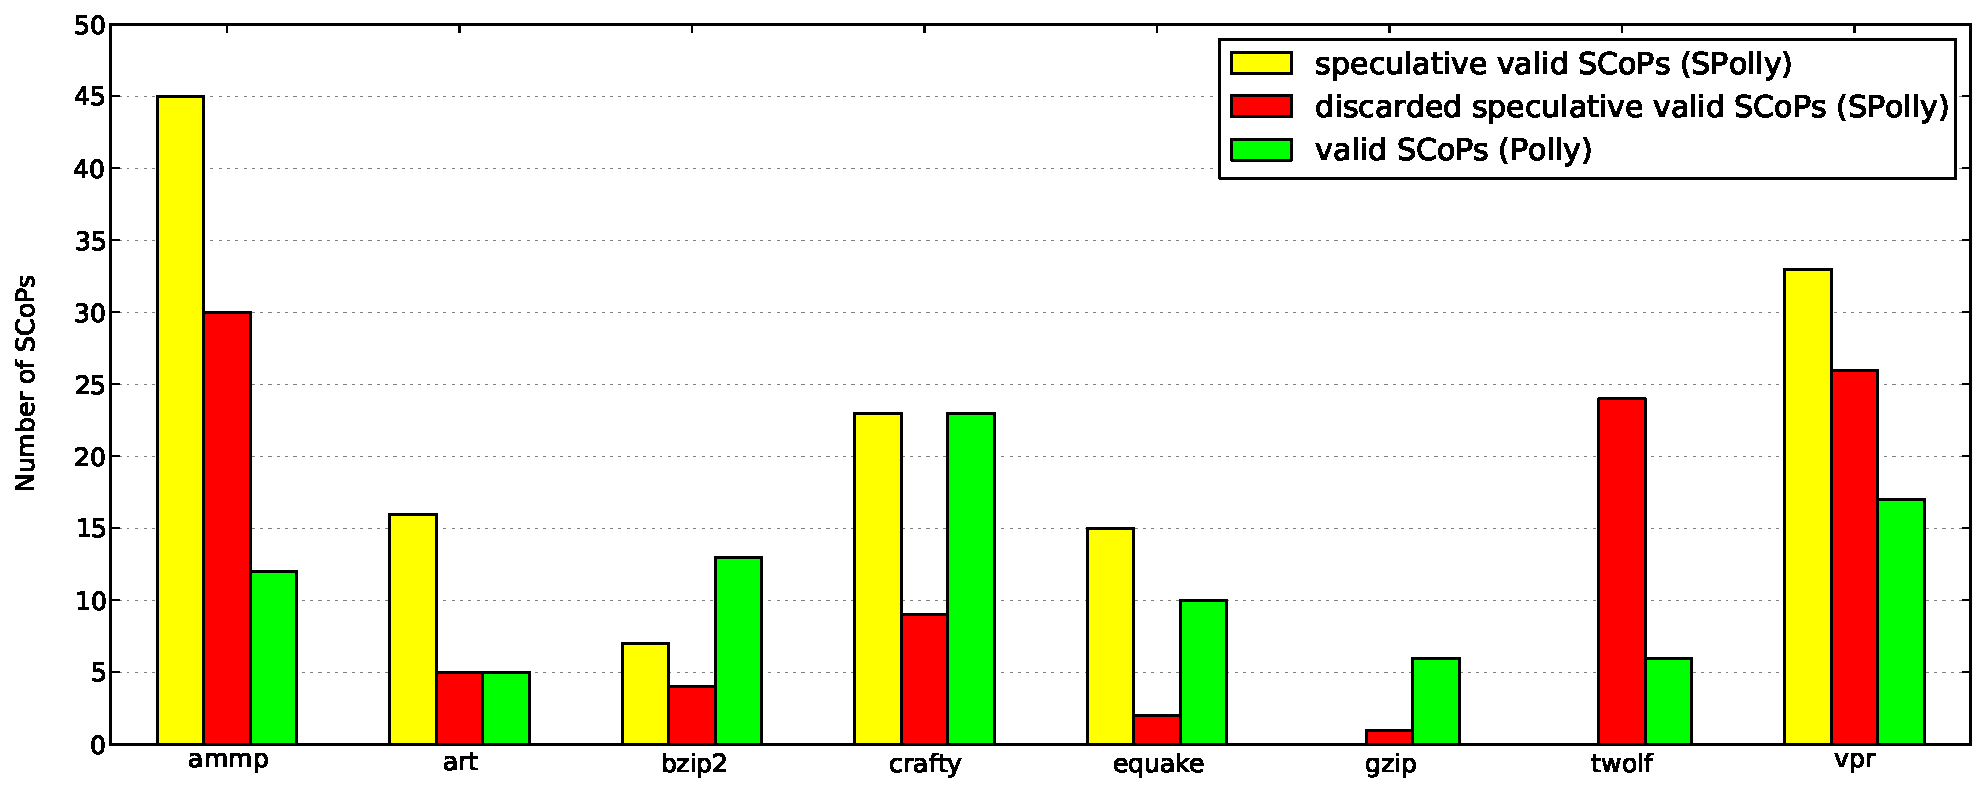
\includegraphics[width=0.9\textwidth]{SPEC2000CT.pdf}
		\rule{35em}{0.5pt}
	\caption{Numbers of valid and speculative valid SCoPs}
	\label{fig:SPEC2000CT}
\end{figure}

\subsubsection{Polybench 3.2}
\begin{figure}[htbp]
	\centering
        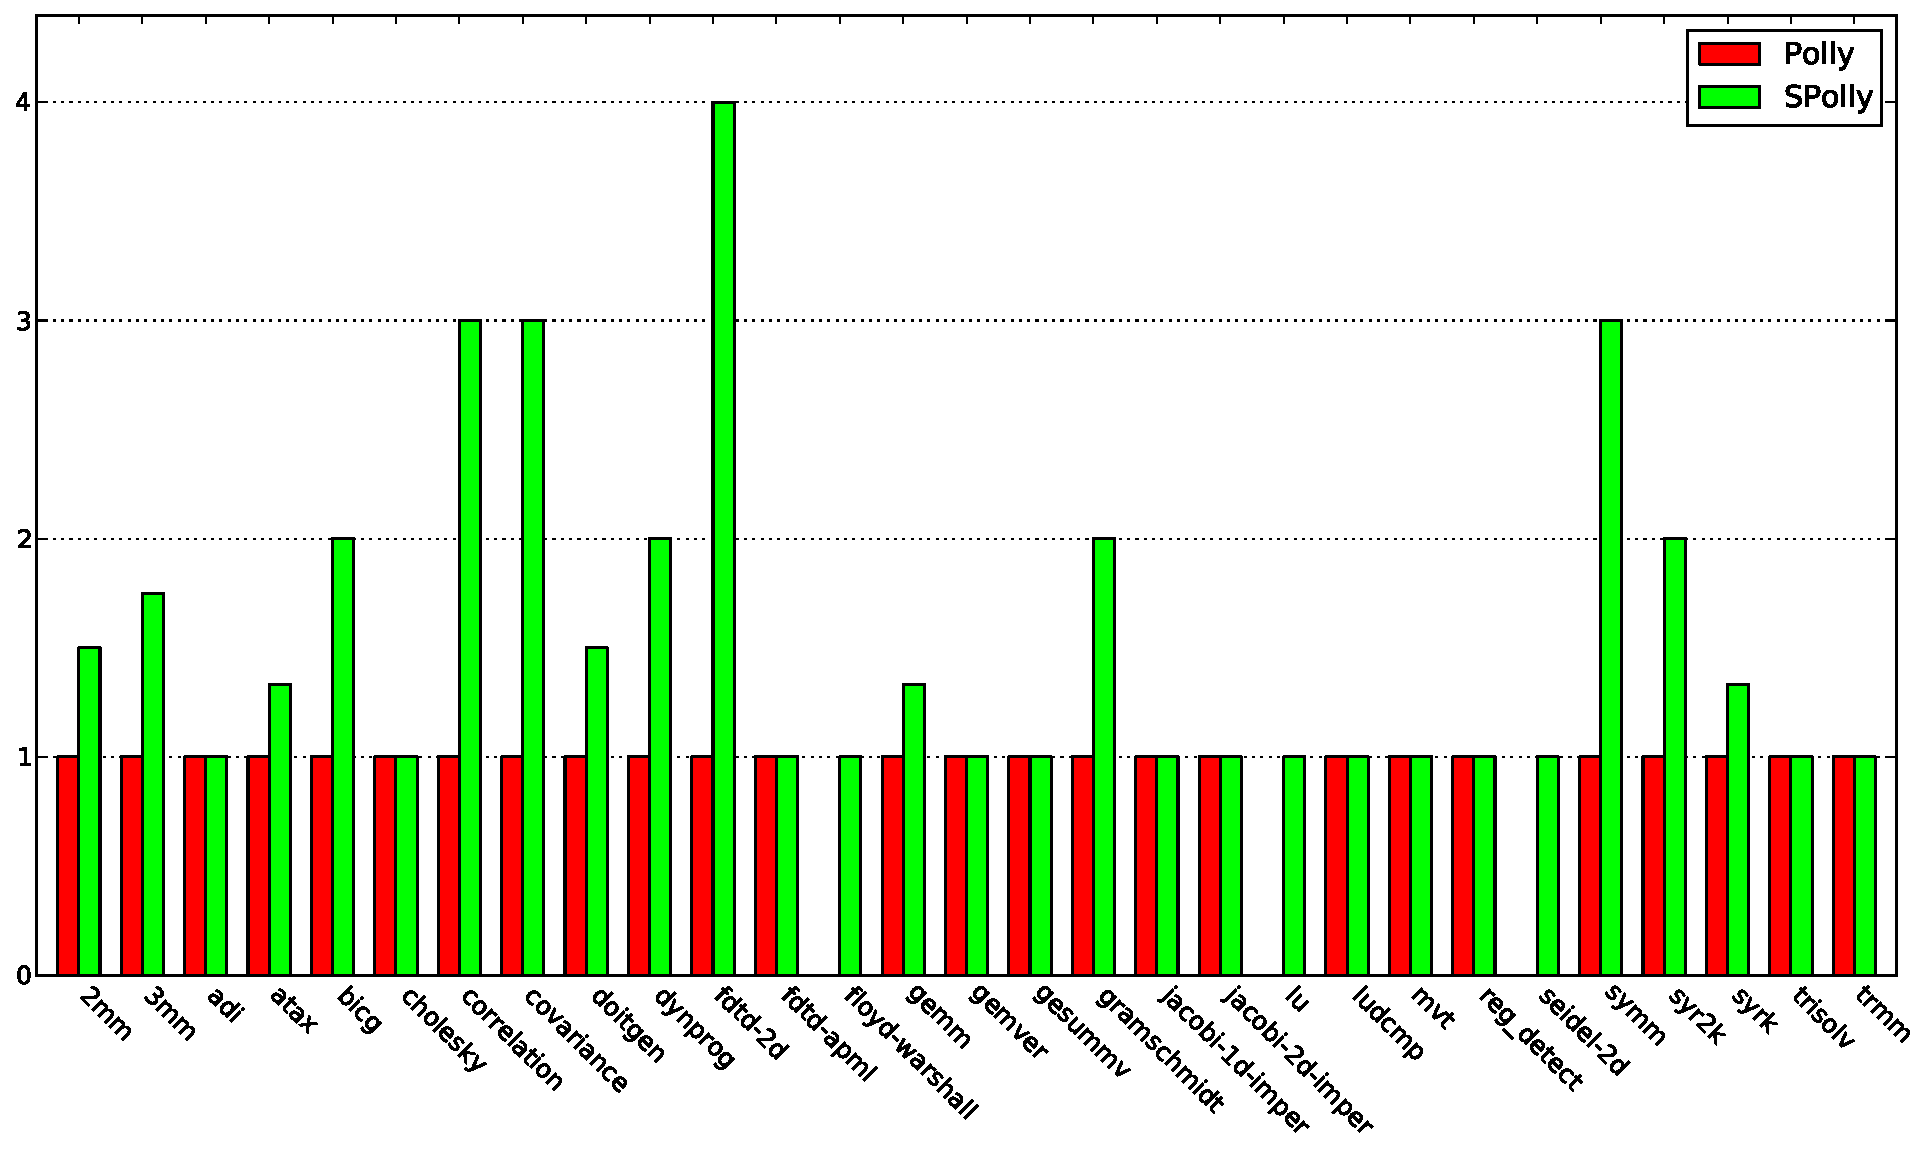
\includegraphics[width=0.9\textwidth]{polybenchCT.pdf}
		\rule{35em}{0.5pt}
	\caption{Numbers of valid and speculative valid SCoPs}
	\label{fig:polybenchCT}
\end{figure}


\begin{figure}[htbp]
	\centering
        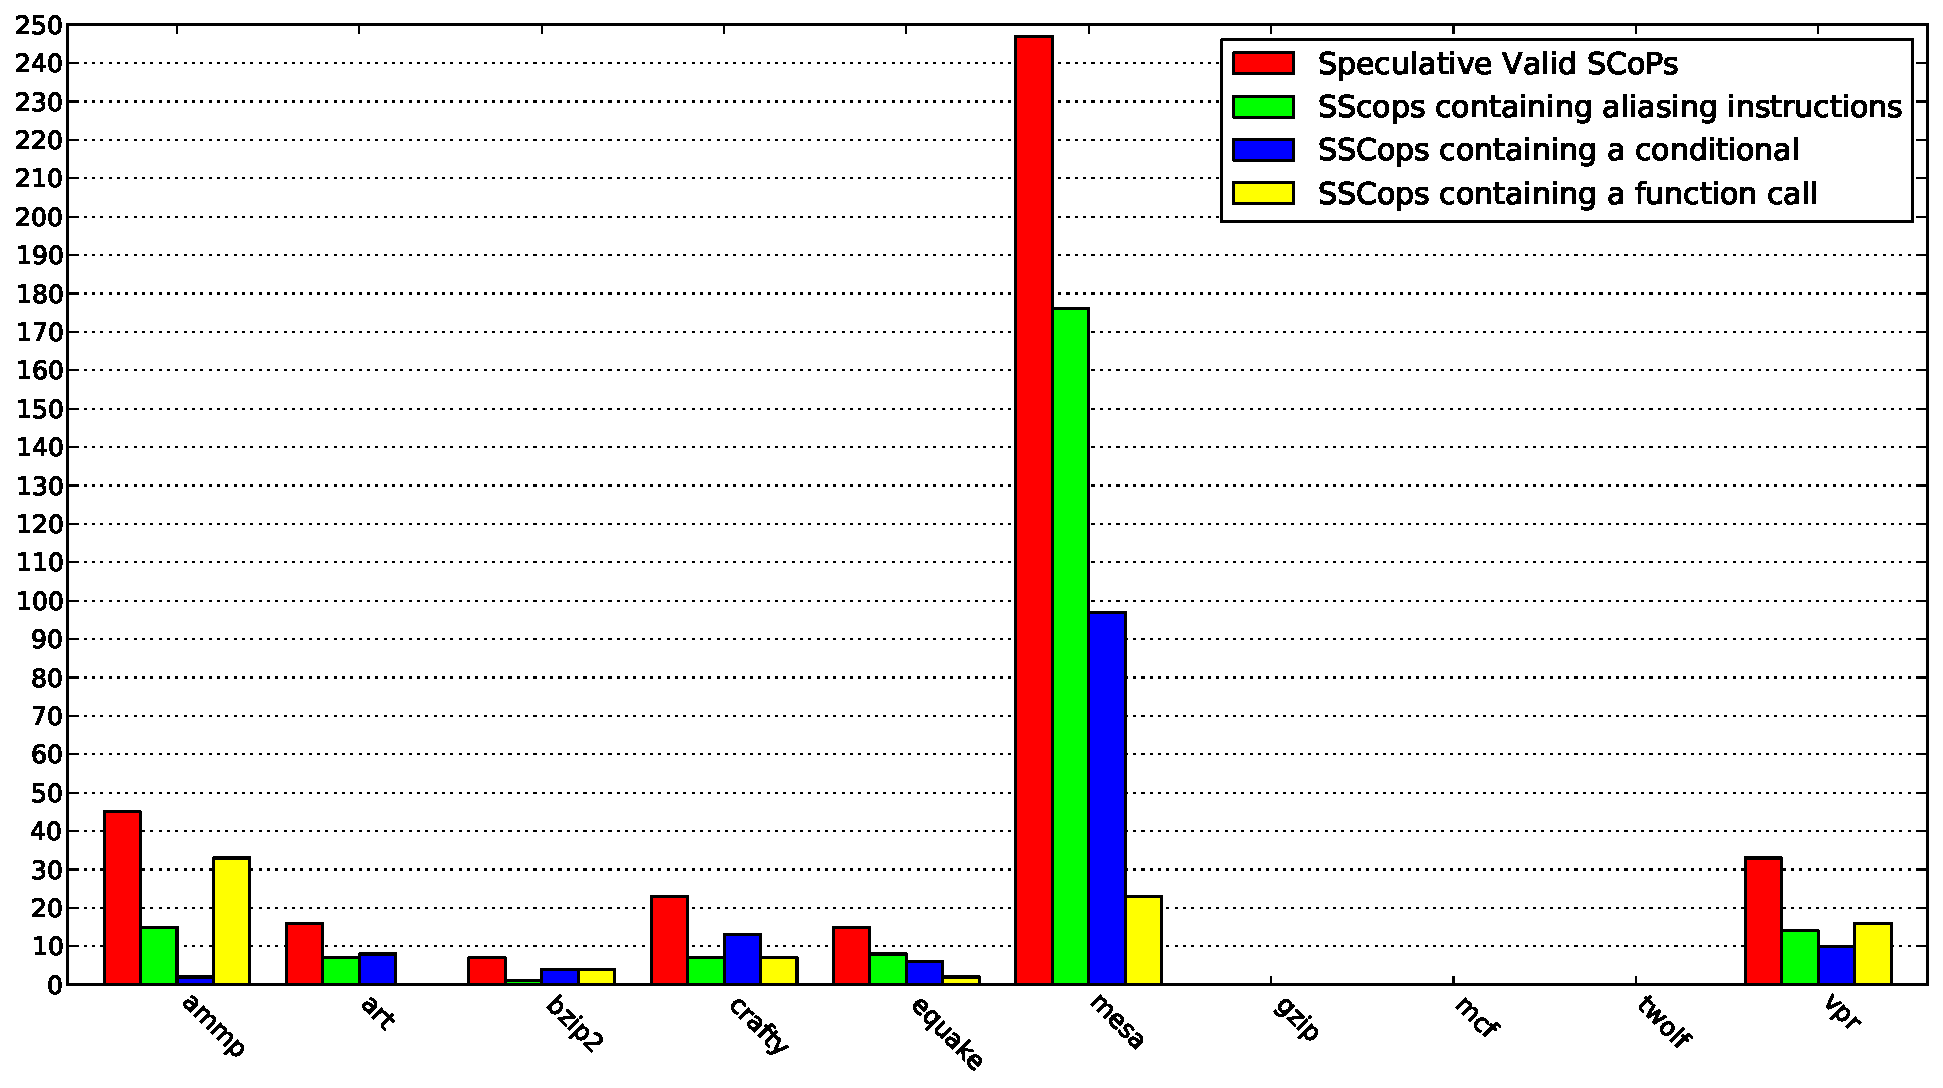
\includegraphics[width=0.5\textwidth]{SPEC2000CTsSCoPsOne.pdf}
		\rule{35em}{0.5pt}
	\caption{Details about speculative valid SCoPs}
	\label{fig:SPEC2000CTsSCoPsOne}
\end{figure}

\subsubsection{Available tests}

\paragraph{Alias tests}


\paragraph{Invariant tests}




\subsection{Sound Transformations}
\label{soundCTtransformations}
As described earlier, region speculation collects violations within a SCoP 
and can introduce tests for some of them. There are cases when these tests will
suffice to get a sound result, thus there is no need for a runtime system at all.
Although this hold in respect to the soundness of a program, this does not mean 
performance will rise when these transformations are used.  \\
TODO scores -- heuristic / statistics 


\section{Runtime Evaluation}


\section{Problems}
During the work with LLVM 3.0 and a corresponding version of Polly a few
problems occurred. Some of them could not be reproduced in newer versions
they were just be tackled with tentative fixes, as they will be resolved as soon
as Sambamba and SPolly will be ported to a newer version.
Others, which could be reproduced in the current trunk versions,
have been reported and listed in figure \ref{tab:bugreports}. All bugs were 
reported with a minimal test case and a detailed description why they occur.

% ID | description | status | patch included | tool
\begin{table}[htbp]
  \caption{Reported bugs}
  \begin{tabularx}{\textwidth}{ c | X | p{2cm} | c | c }
   ID & Description & Status & Patch provided  & Component \\
  \hline \hline
  12426 & Wrong argument mapping in OpenMP subfunctions & RESOLVED FIXED & yes & Polly \\
   \hline
  12427 & Invariant instruction use in OpenMP subfunctions & NEW & yes & Polly \\
   \hline
  12428 & PHInode use in OpenMP subfunctions & NEW & no & Polly \\
   \hline
  TODO & add the others to bugzilla & & & \\
  TODO & PollybenchC2 gemver , 2mm & & & \\
  \end{tabularx}
  \label{tab:bugreports}
\end{table}
 % Evaluation 

% Chapter 5

\chapter{Discussion} % Write in your own chapter title
\label{Chapter5}
\lhead{Chapter 5. \emph{Discussion}} % Write in your own chapter title to set the page header

\section{Quantitative Results}

\section{Qualitative Results}

\section{Interpretation}
 % Results and Discussion

% Chapter 6

\chapter{Case Study} % Write in your own chapter title
\label{Chapter6}
\lhead{Chapter 6. \emph{Case Study}} % Write in your own chapter title to set the page header


\section{Matrix Multiplication}
\label{MatrixMultiplication}
Matrix multiplication is a well known computational problem and part of many 
algorithms. If the data size grows, the runtime may have crucial impact on th
e overall performance. Tiling, vectorization and parallel execution yield an
enormous speedups as different approaches already
showed\cite{grosser:thesis, JIMBOREAN-2012-664345},
still the question about applicability remains. A slightly modified source code 
would not be optimized at all, even if the computation has not been changed. 

This section will compare different implementations of a simple 2d
matrix multiplication. As sample size  $1024*1024$ floats are used 
(\texttt{N} is defined as 1024).
Each example is executed 10 times and the geometric mean of the results 
(without the best and worst one) is computed. All numbers are generated on 
the server described in table \ref{todo}. The base algorithm stays the same 
for each case, so there is no hand made optimization involved. The computed 
result is checked each time in order to prevent false optimizations.


\subsection{Case A}
\begin{wrapfigure}[]{r}{0.5\textwidth}
  \centering
    \begin{minipage}[c]{0.4\textwidth}
    \vspace*{-3mm}
    \lstinputlisting{Primitives/Code/matmul1prep.c}
    \end{minipage}
  \caption{Matmul case A}
   \label{lst:MatmulVersionA}
\end{wrapfigure}

Listing \ref{lst:MatmulVersionA} shows the matrix multiplication as used in 
many presentations and benchmarks. This case is quite grateful because the
global arrays are distinct, the loop nest is perfectly nested and all 
memory accesses can be computed statically. With this in mind the popularity of
this case is hardly surprising, just as the good results of all tested versions 
are.  \\ 




\subsection{Case B}
\begin{wrapfigure}[]{l}{0.5\textwidth}
    \begin{minipage}[c]{0.4\textwidth}
    \vspace*{-3mm}
    \lstinputlisting{Primitives/Code/matmul2prep.c}
    \caption{Matmul case B}
    \end{minipage}
    \label{lst:MatmulVersionB}
\end{wrapfigure}

Listing \ref{lst:MatmulVersionA} shows the matrix multiplication as used in 
many presentations and benchmarks. This case is quite grateful because the
global arrays are distinct, the loop nest is perfectly nested and all 
memory accesses can be computed statically. With this in mind the popularity of
this case is hardly surprising, just as the good results of all tested versions 
are.  \\ 



\subsection{Case C}
\begin{wrapfigure}[]{r}{0.5\textwidth}
  \centering
    \begin{minipage}[c]{0.4\textwidth}
    \vspace*{-3mm}
    \lstinputlisting{Primitives/Code/matmul3prep.c}
    \end{minipage}
  \caption{Matmul case C}
   \label{lst:MatmulVersionC}
\end{wrapfigure}
Listing \ref{lst:MatmulVersionA} shows the matrix multiplication as used in 
many presentations and benchmarks. This case is quite grateful because the
global arrays are distinct, the loop nest is perfectly nested and all 
memory accesses can be computed statically. With this in mind the popularity of
this case is hardly surprising, just as the good results of all tested versions 
are. 


\begin{table}[htpb]

  \caption{Case study results}
  \label{tab:CaseStudyResults}
\end{table}


%\begin{figure}[htpb]
  %\centering
  %\subfloat[Matmul version 1]{

  %} \hfill
  %\subfloat[Matmul version 2]{
    %\begin{minipage}[c]{0.45\textwidth}
    %\lstinputlisting{Primitives/Code/matmul2prep.c}
    %\label{lst:MatmulVersion2}
    %\end{minipage}
  %}

  %\subfloat[Matmul version 3]{
    %\begin{minipage}[c]{0.45\textwidth}
    %\lstinputlisting{Primitives/Code/matmul3prep.c}
    %\label{lst:MatmulVersion3}
    %\end{minipage}
  %}
  %\hfill
  %\subfloat[Matmul version 4]{
    %\begin{minipage}[c]{0.45\textwidth}
    %\lstinputlisting{Primitives/Code/matmul4prep.c}
    %\label{lst:MatmulVersion4}
    %\end{minipage}
  %}
  %\caption{Matrix multiplication in different versions }
%\end{figure}
 % Case study

% Chapter 3

\chapter{The Setup} % Write in your own chapter title
\label{Chapter3}
\lhead{Chapter 3. \emph{The Setup}} % Write in your own chapter title to set the page header


 % Conclusion

%\input{./Chapters/Chapter} % Future work

%% ----------------------------------------------------------------
% Now begin the Appendices, including them as separate files

%% ----------------------------------------------------------------
\clearpage
\lhead{\emph{List of Figures}}  % Set the left side page header to "List if Figures"
\listoffigures  % Write out the List of Figures

\clearpage
%% ----------------------------------------------------------------
\lhead{\emph{List of Tables}}  % Set the left side page header to "List of Tables"
\listoftables  % Write out the List of Tables
\clearpage

%\addtocontents{toc}{\vspace{1em}} % Add a gap in the Contents, for aesthetics
%%% ----------------------------------------------------------------
%\setstretch{1.5}  % Set the line spacing to 1.5, this makes the following tables easier to read
%\clearpage  % Start a new page
%\lhead{\emph{Abbreviations}}  % Set the left side page header to "Abbreviations"
%\listofsymbols{ll}  % Include a list of Abbreviations (a table of two columns)
%{
%% \textbf{Acronym} & \textbf{W}hat (it) \textbf{S}tands \textbf{F}or \\
%\textbf{AA} & \textbf{A}lias \textbf{A}nalysis \\
%\textbf{CFG} & \textbf{C}ontrol \textbf{F}low \textbf{G}raph   \\
%\textbf{cloog} & \textbf{C}hunky \textbf{Loo}p \textbf{G}enerator \\
%\textbf{isl} & \textbf{i}nteger \textbf{s}et \textbf{l}ibrary \\
%\textbf{LOC} & \textbf{l}ines \textbf{o}f \textbf{c}ode   \\
%\textbf{LLVM-IR} & LLVM \textbf{I}ntermediate \textbf{R}epresentation  \\
%\textbf{OpenMP} & \textbf{Open} \textbf{M}ulti-\textbf{P}rocessing   \\
%\textbf{Polly} & \textbf{Poly}hedral \textbf{LL}VM   \\
%\textbf{SCoP} & \textbf{S}tatic \textbf{Co}ntrol \textbf{P}art \\
%\textbf{sSCoP} & \textbf{s}peculative \textbf{S}tatic \textbf{Co}ntrol \textbf{P}art \\
%\textbf{SIMD} & \textbf{S}ingle \textbf{I}nstruction \textbf{M}ultiple \textbf{D}ata   \\
%\textbf{SPolly} & \textbf{S}peculative \textbf{P}olly \\
%\textbf{ParCFG} & \textbf{Par}allel \textbf{CFG}   \\
%}
%% ----------------------------------------------------------------
%\lhead{\emph{List of Listings}}  % Set the left side page header to "List of Listings"
%\renewcommand*{\lstlistingname}{List of Listings}
%\lstlistoflistings % Write out the List of Listings 
%\clearpage


\addtocontents{toc}{\vspace{1em}} % Add a gap in the Contents, for aesthetics

\appendix % Cue to tell LaTeX that the following 'chapters' are Appendices

% Appendix A

\chapter{Matrix Multiplication Example}
\label{AppendixA}
\lhead{Appendix A. \emph{Matrix Multiplication Example}}
	% Appendix Title

% Appendix A

\chapter{SPolly As Static Optimizer Pass}
\label{AppendixB}
\lhead{Appendix B. \emph{SPolly As Static Optimizer Pass}}

\begin{table}[htbp]
  \caption{Command line options to interact with SPolly}
  \begin{tabularx}{\textwidth}{ l p{1mm} X  }
    Command line option     && Description  \\
    \hline
    -enable-spolly          && Enables SPolly during SCoP detection,\par
                                (options containing spolly will not work without) \\ 
    -spolly-replace         && Replaces all sSCoPs by optimized versions \par 
                                (may not be sound)  \\
    -spolly-replace-sound   && As spolly-replace, but sound due to runtime checks \par
                                (iff sound checks can be introduced)\\
    -spolly-extract-regions && Extracts all sSCoPs into their own sub function \\
    -polly-forks=N          && Set the block size which is used when 
                             polly-fork-join code generation is enabled\\
    -enable-polly-fork-join && Extracts the body of the outermost,
                             parallelizeable loop, performs loop blocking with
                             block size N and unrolls the new introduced loop 
                             completely \par
                             (one loop with N calls in the body remains)\\
    -polly-inline-forks     && Inline the call instruction in each fork \\
  \end{tabularx}
  \label{tab:CommandLineOptions}
\end{table}

\begin{table}[htbp]
  \caption{Brief overview of Polly's optimization options}
  \begin{tabularx}{\textwidth}{ l p{1mm} X}
    Short or option name          && Description \\
    \hline
    -polly-no-tiling              && Disable tiling in the scheduler  \\
    -polly-tile-size=N\footnotemark[1] && Create tiles of size N \\
    -polly-opt-optimize-only=STR  && Only a certain kind of dependences (all/raw) \\
    -polly-opt-simplify-deps      && Simplify dependences within a SCoP    \\
    -polly-opt-max-constant-term  && The maximal constant term allowed (in the scheduling) \\
    -polly-opt-max-coefficient    && The maximal coefficient allowed (in the scheduling)  \\
    -polly-opt-fusion             && The fusion strategy to choose (min/max) \\
    -polly-opt-maximize-bands     && Maximize the band depth (yes/no) \\
    -polly-vector-width=N\footnotemark[1]  && Try to create vector loops with N iterations \\
    -enable-polly-openmp          && Enable OpenMP parallelized loop creation \\
    -enable-polly-vector          && Enable loop vectorization (SIMD) \\
    -enable-polly-atLeastOnce     && Indicates that every loop is at leas executed once \\
    -enable-polly-aligned         && Always assumed aligned memory accesses \\
    -enable-polly-grouped-unroll  && Perform grouped unrolling, but don't generate SIMD \\
     &&  \\ 
  \end{tabularx}
  \label{tab:PollyOptions}
  \footnotemark[1] Not available from the command line \\
\end{table}


 % Appendix Title

%\input{./Appendices/AppendixC} % Appendix Title

\addtocontents{toc}{\vspace{2em}}  % Add a gap in the Contents, for aesthetics
\backmatter

%% ----------------------------------------------------------------
\label{Bibliography}
\hypersetup{urlcolor=Maroon}  % Colours hyperlinks in blue, but this can be distracting if there are many links.
\lhead{\emph{Bibliography}}  % Change the left side page header to "Bibliography"
\bibliographystyle{unsrtnat}  % Use the "unsrtnat" BibTeX style for formatting the Bibliography
\bibliography{Bibliography}  % The references (bibliography) information are stored in the file named "Bibliography.bib"

\end{document}  % The End
%% ----------------------------------------------------------------
